%%%%%%%%%%%%%%%%%%%%%%%%%%%%%%%%%%%%%%%%%
% The Legrand Orange Book
% LaTeX Template
% Version 2.0 (9/2/15)
%
% This template has been downloaded from:
% http://www.LaTeXTemplates.com
%
% Mathias Legrand (legrand.mathias@gmail.com) with modifications by:
% Vel (vel@latextemplates.com)
%
% License:
% CC BY-NC-SA 3.0 (http://creativecommons.org/licenses/by-nc-sa/3.0/)
%
% Compiling this template:
% This template uses biber for its bibliography and makeindex for its index.
% When you first open the template, compile it from the command line with the
% commands below to make sure your LaTeX distribution is configured correctly:
%
% 1) pdflatex main
% 2) makeindex main.idx -s StyleInd.ist
% 3) biber main
% 4) pdflatex main x 2
%
% After this, when you wish to update the bibliography/index use the appropriate
% command above and make sure to compile with pdflatex several times
% afterwards to propagate your changes to the document.
%
% This template also uses a number of packages which may need to be
% updated to the newest versions for the template to compile. It is strongly
% recommended you update your LaTeX distribution if you have any
% compilation errors.
%
% Important note:
% Chapter heading images should have a 2:1 width:height ratio,
% e.g. 920px width and 460px height.
%
%%%%%%%%%%%%%%%%%%%%%%%%%%%%%%%%%%%%%%%%%

%----------------------------------------------------------------------------------------
%	PACKAGES AND OTHER DOCUMENT CONFIGURATIONS
%----------------------------------------------------------------------------------------

\documentclass[12pt,fleqn]{book} % Default font size and left-justified equations

%----------------------------------------------------------------------------------------

\input{structure} % Insert the commands.tex file which contains the majority of the structure behind the template
\definecolor{light-gray}{gray}{0.95}
\newcolumntype{g}{>{\columncolor{light-gray}}p{4cm}}

\usepackage[printwatermark]{xwatermark}
\newwatermark[allpages,color=gray!50,angle=45,scale=4,xpos=0,ypos=0]{DRAFT}

\begin{document}

%----------------------------------------------------------------------------------------
%	TITLE PAGE
%----------------------------------------------------------------------------------------

\begingroup
\thispagestyle{empty}
\begin{tikzpicture}[remember picture,overlay]
\coordinate [below=8cm] (midpoint) at (current page.north);
\node at (current page.north west)
{\begin{tikzpicture}[remember picture,overlay]
\node[anchor=north west,inner sep=0pt] at (0,0) {\includegraphics[width=\paperwidth]{background1}}; % Background image
\draw[anchor=north] (midpoint) node [fill=ocre!30!,fill opacity=0.6,text
opacity=1,inner
sep=1cm]{\Huge\centering\bfseries\sffamily\parbox[c][][t]{\paperwidth}{\centering
    Distributed Hosting\\[15pt] % Book title
{\Large A Blockchain Based Distributed Hosting Engine}\\[20pt] % Subtitle
{\normalsize Alex Oberhauser, Stavros Champilomatis, Nikos Sarris and Maria Efthimiadou}}}; % Author name
\end{tikzpicture}};
\end{tikzpicture}
\vfill
\endgroup

%------------------------------------------------------------------------------
%	COPYRIGHT PAGE
%------------------------------------------------------------------------------

\newpage
~\vfill
\thispagestyle{empty}

\noindent Copyright \copyright\ 2015 The BlackGate Team\\ % Copyright notice

\noindent \textsc{Published by the \textit{BlackGate} Team}\\ % Publisher

\noindent \textsc{http://blackgate.networld.to}\\ % URL

\noindent This work is licensed under the Creative Commons Attribution 4.0 International License. To view this license visit \url{http://creativecommons.org/licenses/by/4.0/}.\\ % License information

\noindent \textit{First released, March 2015} % Printing/edition date

%------------------------------------------------------------------------------
%	TABLE OF CONTENTS
%------------------------------------------------------------------------------

\chapterimage{chapter_head_1.pdf} % Table of contents heading image

\pagestyle{empty} % No headers

\tableofcontents % Print the table of contents itself

\cleardoublepage % Forces the first chapter to start on an odd page so it's on the right

\pagestyle{fancy} % Print headers again

%------------------------------------------------------------------------------
%	PART
%------------------------------------------------------------------------------
\part{Overview}

%------------------------------------------------------------------------------
%	CHAPTER 1
%------------------------------------------------------------------------------

\chapterimage{chapter_head_2.pdf} % Chapter heading image

\chapter{Introduction}
% -*- root: ../distributed_hosting_whitepaper.tex -*-

This part gives a motivation and a general overview about the
\textit{Distributed Hosting Engine}. It introduces some concepts that will be
explained in more detail in the next part. If you are looking for a detailed specification you can directly go to Part \ref{part:specifications}.

\section{Hosting Paradigm Shift}\index{Hosting Paradigm Shift}

This whitepaper specifies a new protocol and blockchain that has
the potential to change the current hosting paradigm. Instead of retrieving
pages from a specific location, they are hosted directly on end-user
devices. The distributed hosting algorithm and protocol, specified here, takes
care of the optimal location for each page. By taking into account different
metrics, like response times, availability and/or relevance, the perfect place
for each page will be found after some time. This not only increases the
performance for single page accesses, but reduced also network load and hence
increases the overall network health.

Additional to the increased performance, the underlying blockchain assures the
correctness and validity of each page, also, or especially, if hosted by a
random node in the network. This validation mechanism is then used to create a
reputation system, allowing blocking of malicious nodes that have a reputation
score that is lower than a threshold value.

This mechanism, together with the page distribution algorithm, makes the
network self-managing, self-healing and robust against changes.

By design the \textit{Distributed Hosting Engine} is censorship resistance,
but only under the assumption that there are enough nodes that are willing to
host the page. This moves responsibility what could be hosted from a central
authority to the collective.

From a commercial point of view the here proposed approach allows the creation
of an interoperable hosting ecosystem. Each hosting provider acts as clone and
has no direct access to the page, but can support the user with additional
(paid or free) services and hosting space. By design a switch from one
hosting provider to another one does not affect the hosting of the page, nor
the page itself. Technical there is not even a migration happening, only a
switch from one page creation tool to another one.

\section{Use Cases}\index{Use Cases}

\textbf{TODO:} Explains here different use cases based on user stories of Jane
and John Doe.


\chapterimage{chapter_head_4.pdf} % Chapter heading image

\chapter{Empowering Technology}
% -*- root: ../distributed_hosting_whitepaper.tex -*-

This chapter explains the technologies that make the \textit{Distributed
Hosting Engine} possible. Most notable the concept of \textit{Blockchains} for
the distributed management and self-organization of pages and \textit{Tor
Hidden Services} that not only protect the privacy of all involved parties,
but that also allows to host pages behind NATs and Firewalls.

\section{Blockchain}\index{Blockchain}

\textit{Blockchain} is a rather new concept, with a lot of potential. A
\textit{Blockchain} is a distribute ledgers that prevents double spending without a central authority. The first time the \textit{Blockchain} was mentioned and implemented was for Bitcoin \cite{nakamoto2008bitcoin}.

\section{Tor Hidden Services}\index{Tor Hidden Services}

Tor hidden services are generally used to host pages anonymously and protect
visitors and hosters alike. In the scope of this whitepaper tor hidden
services are used to enable hosting from everywhere, no matter if the device
is behind a NAT or a Firewall. This allows to host pages from public wireless
hotspots, from the office or from home. Without the possibility to abstract
away from public accessible IPs and the capability to circumvent Firewalls it
would not be possible to develop real distributed hosting on end-user devices.


\chapterimage{chapter_head_5.pdf} % Chapter heading image

\chapter{Ecosystem}
% -*- root: ../distributed_hosting_whitepaper.tex -*-

\section{Hosting Provider}\index{Hosting Provider}

\textbf{TODO:} Explain here the role change of hosting providers. For example:
A hosting provider does provide service on top of the blockchain, like page
generators and frontends for page publications and updates. If a hosting
provider decides to host a page, it is only one clone out of many without
special role.

\section{Complementary Services}\index{Complementary Services}

\textbf{TODO:} Figure out what alternatives services could be provided by the
ecosystem. This includes also new business ideas for new types of startups.



%------------------------------------------------------------------------------
%	PART
%------------------------------------------------------------------------------
\part{Specifications}\label{part:specifications}

%------------------------------------------------------------------------------
%	CHAPTER 2
%------------------------------------------------------------------------------

\chapterimage{chapter_head_3.pdf} % Chapter heading image

\chapter{Blockchain Specification}

\section{Transaction Definition}\index{Transaction Definition}
% -*- root: ../distributed_hosting_whitepaper.tex -*-

This section defines transactions and their relationship to each other and to
external data. It also defines a (de-)serialization format to and
from the binary format that is transferred over the wire. In Figure
\ref{fig:transactions} a chain of transactions, with relevant fields, is
shown. This example includes three hosts that have cloned the page and in total
three updates.

\begin{figure}[htp]
\includegraphics[width=\textwidth]{transactions.png}
\label{fig:transactions}
\caption{Transaction chain example for one page.}
\end{figure}

\subsection{Transaction Definition}

Update transactions can only be created by the page creator. Additional to the
proof of ownership they also include a reference to the new content, with
related checksums.

\begin{table}[ht]
  \centering
  \begin{tabular}{|g|p{10cm}|}
    \hline
    \multicolumn{2}{|c|}{\textbf{TRANSACTION HEADER}}\\
    \hline
    \textbf{TransactionID} & Double SHA256 hash of this transaction.\\
    \hline
    \textbf{Parent} & The previous update \textit{TransactionID}\\
    \hline
    \textbf{ScriptSig} & \textbf{TODO Future Work:} Proof here ownernship of
    the hostname and all requirements that come with this update.\\
    \hline
    \textbf{Hostname} & The tor hidden service onion hostname of this page.
    Tor hidden services are needed to be able to host page behind firewalls
    and NATs. Additional they protect the identity of the content owner and
    more importantly of clone hosts.\\
    \hline
    \multicolumn{2}{|c|}{\textbf{CONTENT SECTION}}\\
    \hline
    \textbf{Snapshot} & The hash value of the content. This hash value is used
    to find all peers in the Distributed Hash Table (DHT) that share currently
    this snapshot. The DHT is bootstrapped by using all active hostname in the
    blockchain. For increased compatibility the MAGNET URI scheme is used.\\
    \hline
    \textbf{SnapshotChecksum} & Checksum of the Snapshot content, used to
    verify the downloaded data.\\
    \hline
    \textbf{ResponseChecksum} & Checksums for all endpoints of this page.
    Makes each page verifiable and hence could be served by a random node. If
    the returned content does not match the here checksum the response is
    invalid.\\
    \hline
    \textbf{Flags} & \textbf{TODO Future Work:} Could be used for
    differentiation between incremental and full updates, but also indicating
    that this page is not hosted anymore and could be deleted.\\
    \hline
  \end{tabular}
\end{table}

\subsection{CLONE Transaction Definition}

\textbf{TODO:} This transaction can be merge with the UPDATE transaction. They
do not differ too  much, except that they have different Flags content and
that the CLONE transaction does not include all fields.

Clone transactions are created and propagated by all hosts that start hosting
a page or if they receive a new update transaction. This transactions always
link back to exactly one update transaction.

\begin{table}[ht]
  \centering
  \begin{tabular}{|g|p{10cm}|}
    \hline
    \textbf{TransactionID} & Double SHA256 hash of this transaction.\\
    \hline
    \textbf{Parent} & The previous update \textit{TransactionID}\\
    \hline
    \textbf{ScriptSig} & \textbf{TODO Future Work:} Proof here ownernship of
    the hostname and all requirements that come with this update.\\
    \hline
    \textbf{Hostname} & The tor hidden service onion hostname of this page.
    Tor hidden services are needed to be able to host page behind firewalls
    and NATs. Additional they protect the identity of the content owner and
    more importantly of clone hosts.\\
    \hline
    \textbf{Flags} & Possible values are: \textit{CLONE} when new update was
    received or \textit{PURGE} if the page is not hosted anymore.\\
    \hline
  \end{tabular}
\end{table}


\section{Block Definition}\index{Block Definition}
\textbf{TODO:} Define here the block as transmitted via the network and how it
will be stored (slightly different).


\section{Mining Process}\index{Mining Process}
% -*- root: ../distributed_hosting_whitepaper.tex -*-

\textbf{Note:} \textit{This section is work in progress. The resulting
description is a first naive solution. Currently in discussion are multi-
entity ownerships and a consensus network between this small group of page
owners, e.g. with Practical Byzantine Fault Tolerance (PBFT)
\cite{castro1999practical}.}

By definition each page in the hosting space has an own blockchain. In the
\textit{Genesis Block} the \textit{Content Creator} proofs ownership of this
blockchain and hence the related page. The assumption here is that only the
\textit{Content Creator} can update the page and that (s)he is the only entity
that has not intention to compromise the own page.


%----------------------------------------------------------------------------------------
%	CHAPTER 3
%----------------------------------------------------------------------------------------
\chapter{Protocol Specification}

In Figure \ref{fig:data_cloud_blockchain} the relationship between the page
content (html, css, javascript, images...), in the middle cloud, the data
(above) and blockchain overlay network (below) is shown. The network that
manages the page content has not to be the same as the blockchain network, but
they maybe nearly identical or overlapping. The page content is not part of
the blockchain, but referenced from it. This allows to have no page content
size limit and the data exchange could be optimized.

\begin{figure}[htp]
\centering
\includegraphics[width=0.75\textwidth]{pictures/data_cloud_blockchain.png}
\caption{Relationship between blockchain and page content from a network
perspective.}
\label{fig:data_cloud_blockchain}
\index{Overlay Networks Figure}
\end{figure}

\section{Blockchain Overlay Network}\index{Blockchain Overlay Network}
% -*- root: ../distributed_hosting_whitepaper.tex -*-

The blockchain overlay network consists of nodes that are responsible for
blockchain exchanges. Each nodes keeps track of a set of blockchains,
dependent on the surfing behaviour of the user. Each blockchain includes a
list of known nodes that are used to keep track of updates insides this
blockchain. As a matter of fact it is valid to say that the overall network
consists of multiple overlay networks, one for each blockchain or page.

After extracting the original host and all co-hosts from a blockchain, the
node keeps track about the performance of each found node and prioritises
them. For the prioritisation quality of service properties, like availability
or correctness of received information, are used. The highest ranking nodes
are used to keep track about updates and propagate changes.

If a blockchain is known, new nodes can be found by extracting them from the
propagated \textit{CLONE} transactions. If the blockchain is not yet known,
the node accesses the page for the first time, there are not fallback nodes if
the original host is offline. For that specific node the page looks like if it
is offline, also if there enough co-host to satisfy the request.

\subsection{\color{red}{[REJECTED] Solution 1: Global Blockchain}}

One solution to this problem is to introduce a global blockchain that keeps
track of all page blockchains. By using the sidechain approach
\cite{back2014enabling}, the page blockchains could be linked against the
global blockchain. Each time a new co-hosts starts hosting a page and
propagates a CLONE transaction, in one of the sidechains, the global
blockchain  keeps track of this change and adds this host to a list of co-
hosts related to the sidechain. Without going into detail how this could be
specified and implemented, there are some problems with this approach.

\paragraph{Dynamic Nature}
In difference to the Bitcoin and other blockchains our
approach relies on an external state that can not be usefully modelled in
transactions, through the high frequency of changes, and that is the
availability of co-hosts. Co-hosts are only relevant if they are online at a
given point in time. Keeping track of availability of nodes in a global
blockchain is not only counter productive, but also infeasible. A solution
would be to keep track of all co-hosts and let figure out the nodes what to
node to contact. This makes it pretty inefficient if the sidechain grows.

\paragraph{Scalability issue of block generation}
The Bitcoin mining approach to
solve the scalability problem by hashing power and changing complexity based
on the networks' computation power is not suitable in this case. The here
presented blockchain has no underlying asset that has to be mined. This makes
the proof of work a waste of energy and time. For the same reason proof
of stake is also not suitable. The mentioned approaches in literature are
suitable from a theoretical point of view, but are not able to scale,
e.g. \citetitle{castro1999practical} \cite{castro1999practical}.

\subsection{\color{green}{[ACCEPTED] Solution 2: Distributed Hash Table lookup}}

An alternative solution is to avoid a global blockchain altogether and instead
keep track of co-hosts, related to the original page host, inside a
\textit{Distributed Hash Table (DHT)}. For page content, aka. snapshots,
distributions a DHT is used to lookup which node has currently the needed
snapshot. After that the BitTorrent protocol is used to download and then
distributed the content further. With minimal or no modifications at all the
same approach can be used to lookup co-hosts, that are related to an original
page host.

Every node in all blockchains is also part of this DHT and can be hence used as
entry point for lookups for all other blockchains. If a host does not have any
blockchains at all, publicly known hosts can be used as entrypoints. These
entrypoints should be maintained by the community.

\begin{figure}[htp]
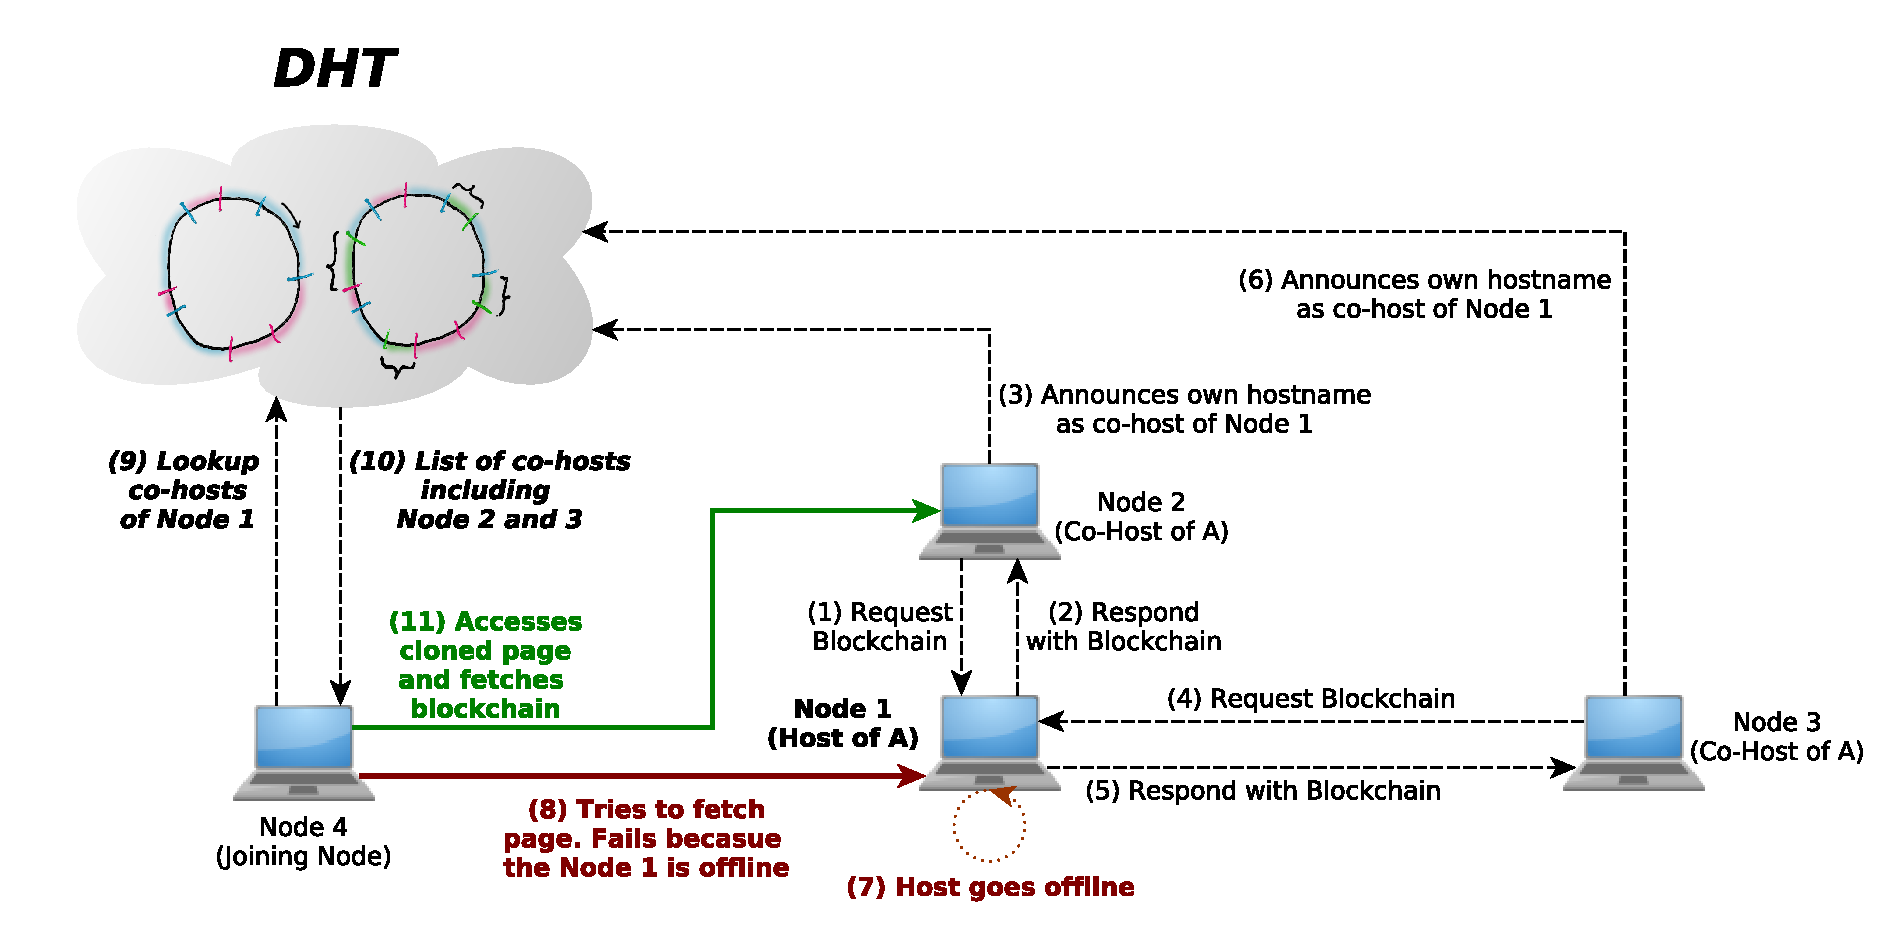
\includegraphics[width=\textwidth]{pictures/dht_solution_to_first_lookup.pdf}
\caption{Proposed solution, based on a Distributed Hash Table (DHT) for the
first lookup problem if the original host is offline.}
\label{fig:dht_solution}
\end{figure}

Figure \ref{fig:dht_solution} explains that approach. \textit{Node 1} is the
content creator and hosts a page. \textit{Node 2} and \textit{3} access the
page, fetch the blockchain and start hosting. After propagating a
\textit{CLONE} transaction to the network, they also announce themselves to
the DHT. Each time they continue hosting, e.g. coming back online,
an announce messages is send. \textit{Node 4} wants to access the page of
\textit{Node 1}, but this node is currently offline. By looking up all,
currently online co-hosts \textit{Node 4} can choose in this example between
\textit{Node 2} or \textit{3}, it chooses \textit{Node 2}.

\section{Data Overlay Network}\index{Data Overlay Network}
\section{Hosting Algorithm}\index{Hosting Algorithm}
\section{Node Handling}\index{Node Handling}
All nodes assign priorities to its neighbor nodes in the overlay network.
The priority, which is a subjective metric, represents ratio of the response
messages, Transaction or a Block, requested from a specific host to the
overall responses (from all the hosts). \\
$score = \frac{receivedTransaction + receivedBlock}{allResponses}$



The host, which receives the response message, increments always the allResponses value but
only the receivedTransaction or receivedBlock one for the host whose message
arrived first.


%------------------------------------------------------------------------------
%	PART
%------------------------------------------------------------------------------
\part{Appendix}

%------------------------------------------------------------------------------
%	BIBLIOGRAPHY
%-----------------------------------------------------------------------------
\chapterimage{chapter_head_6.pdf} % Chapter heading image
\chapter*{Bibliography}
\addcontentsline{toc}{chapter}{\textcolor{ocre}{Bibliography}}
%\section*{Books}
%\addcontentsline{toc}{section}{Books}
%\printbibliography[heading=bibempty,type=book]
%\section*{Articles}
%\addcontentsline{toc}{section}{Articles}
%\addcontentsline{toc}{section}{Articles}
%\printbibliography[heading=bibempty,type=article]
%\nocite{*}
\printbibliography[heading=bibempty]

%----------------------------------------------------------------------------------------
%	INDEX
%----------------------------------------------------------------------------------------

\cleardoublepage
\phantomsection
\setlength{\columnsep}{0.75cm}
\addcontentsline{toc}{chapter}{\textcolor{ocre}{Index}}
\printindex

%----------------------------------------------------------------------------------------

\end{document}
